\documentclass[12pt,letterpaper]{article}
\usepackage{fullpage}
\usepackage[top=2cm, bottom=4.5cm, left=2.5cm, right=2.5cm]{geometry}
\usepackage{amsmath,amsthm,amsfonts,amssymb,amscd}
\usepackage{lastpage}
\usepackage{enumerate}
\usepackage{fancyhdr}
\usepackage{mathrsfs}
\usepackage{xcolor}
\usepackage{graphicx}
\usepackage{listings}
\usepackage{hyperref}
\usepackage{enumitem}
\usepackage[export]{adjustbox}
\graphicspath{ {./images/} }


\lstdefinestyle{Python}{
    language        = Python,
    frame           = lines, 
    basicstyle      = \footnotesize,
    keywordstyle    = \color{blue},
    stringstyle     = \color{green},
    commentstyle    = \color{red}\ttfamily
}

\setlength{\parindent}{0.0in}
\setlength{\parskip}{0.05in}

% Edit these as appropriate
\newcommand\course{CSE 1505}
\newcommand\hwnumber{2}                  % <-- homework number
\newcommand\NetIDa{-}           % <-- NetID of person #1
\newcommand\NetIDb{-}           % <-- NetID of person #2 
\newcommand\NetIDc{-}


\pagestyle{fancyplain}
\headheight 35pt
\lhead{\NetIDa \\ \NetIDb \\ \NetIDc}

 % <-- Comment this line out for problem sets (make sure you are person #1)
\chead{\textbf{\Large Homework \hwnumber}}
\rhead{\course \\ \today}

\lfoot{}
\cfoot{}
\rfoot{\small\thepage}
\headsep 2.5em

\begin{document}

\section*{Task 1: Relational Algebra}
\begin{enumerate}
    \item $\Pi_{Fname, Lname} \sigma_ {Fname = Dependent\_name}(EMPLOYEE \times DEPENDENT)$
    
    \item $\Pi_{e.Fname, e.Lname}(\\
    \rho \ e \ EMPLOYEE \bowtie e.Super\_ssn = s.Ssn \\
    \sigma_{s.Fname = 'James' \ \wedge \ s.Lname = 'Borg'} \  \rho \ s \ EMPLOYEE)$
    
    \item $\Pi_{Fname, Lname}(\\
    \sigma_{e.Dno = 5} \ \rho \ e \ EMPLOYEE \bowtie w.Essn = e.Ssn\\
    (\sigma_{w.Hours > 5} ( \rho \ w \ WORKS\_ON)) \bowtie p.Pnumber = w.Pno \\
    ( σ p.Pname = 'ProductX' \ ( \rho \ p \ PROJECT) \ )
    \\)$
    
    \item $\Pi_{Pname, total\_hours\_week \ \gamma \ Pname}$$_{;}$ $_{SUM(Hours) \rightarrow total\_hours\_week}\\
    (\sigma_{Pnumber = Pno} (PROJECT \times WORKS\_ON))$
    
    \item 
    \end{enumerate}

\section*{Task 2: Logical Schema Design}
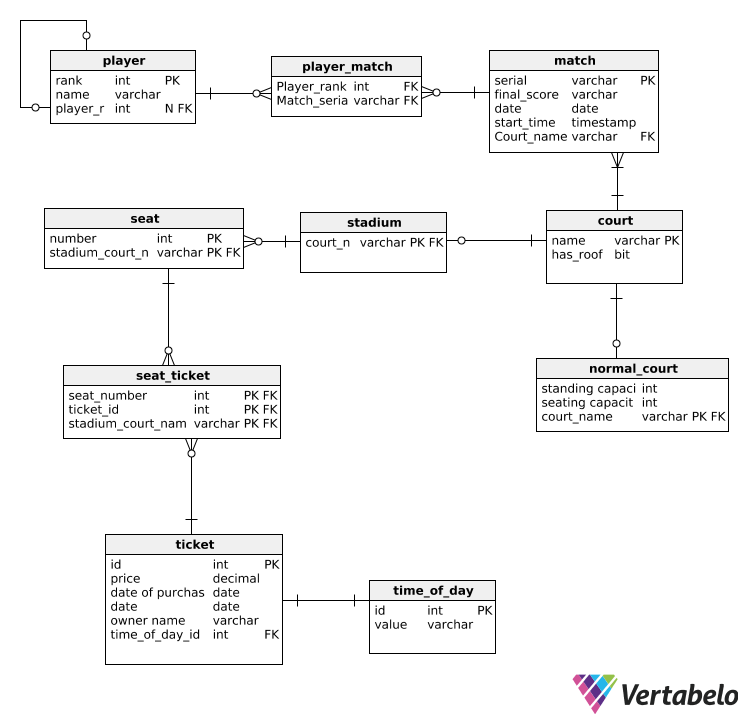
\includegraphics[width=1.0\textwidth, center]{images/Task2.png}
\newpage

\section*{Task 3: Functional Dependencies}
\begin{enumerate}[label={3.\arabic*},nolistsep,leftmargin=*]
\item
    \textbf{CUSTOMER} \\
    \{CCODE\} $\longrightarrow$ \{CNAME, SSN, CADDR, CMAIL, CPHONE, BDATE, SEX\}\\
    \{SSN\} $\longrightarrow$ \{CNAME, CCODE, CADDR, CMAIL, CPHONE, BDATE, SEX\}
    
    \textbf{BRANCH} \\
    \{BCITY, BADDR\} $\longrightarrow$ \{BCODE, BMAIL, BPHONE\}\\
    \{BCODE\} $\longrightarrow$ \{BCITY, BADDR, BMAIL, BPHONE\}
    
    \textbf{LOAN}\\
    \{LNUM\} $\longrightarrow$ \{LAMOUNT, LCUSTOMER, LBRANCH\}
    
    \textbf{PAYMENT}\\
    \{PNUM, PLOAN\} $\longrightarrow$ \{PDATE, PAMOUNT, PBRANCH\}\\

\item
    \textit{Customer\_Rel}(\underline{CCODE}, \underline{SSN}, CNAME, CADDR, CMAIL, CPHONE, BDATE, SEX )
    
    \textit{Branch\_Rel}(\underline{BCITY, BADDR}, \underline{BCODE}, BMAIL, BPHONE)
    
    \textit{Loan\_Rel}(\underline{LNUM}, LCUSTOMER $\longrightarrow$ \textit{Customer}(CCODE), LBRANCH $\longrightarrow$ \textit{Branch}(BCODE), LAMOUNT)
    
    \textit{Payment\_Rel}(\underline{PNUM, PLOAN} $\longrightarrow$ \textit{Loan}(LNUM) , PBRANCH $\longrightarrow$ \textit{Branch}(BCODE), PDATE, PAMOUNT)
    
\end{enumerate}

\section*{Task 4: Normalization}

\begin{enumerate}[label={4.\arabic*},nolistsep,leftmargin=*]
  \item
   This relation is in 1NF because the non-key attribute title depends only on the course\textunderscore id which is a proper subset of the composite key: course\textunderscore id, sec\textunderscore id, semester, year.
  \item
    2NF: Removed all non-key attributes that depend on a proper subset of the composite key.  \\
    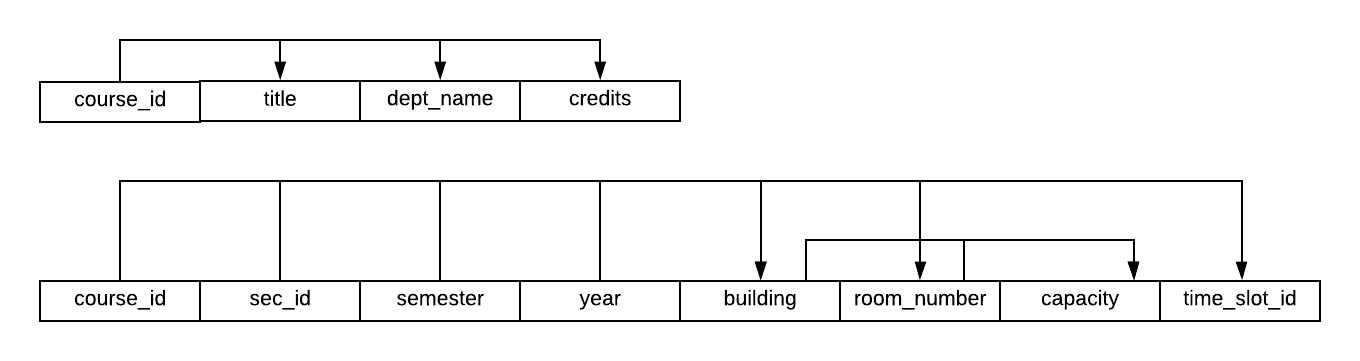
\includegraphics[width=1.0\textwidth, center]{images/2NF.png}
    
    \newpage
    3NF: The attribute \textit{capacity} is in 2NF determined by two keys. Therefore we've created another table so that every non-key attribute is only determined by the candidate key.  \\
    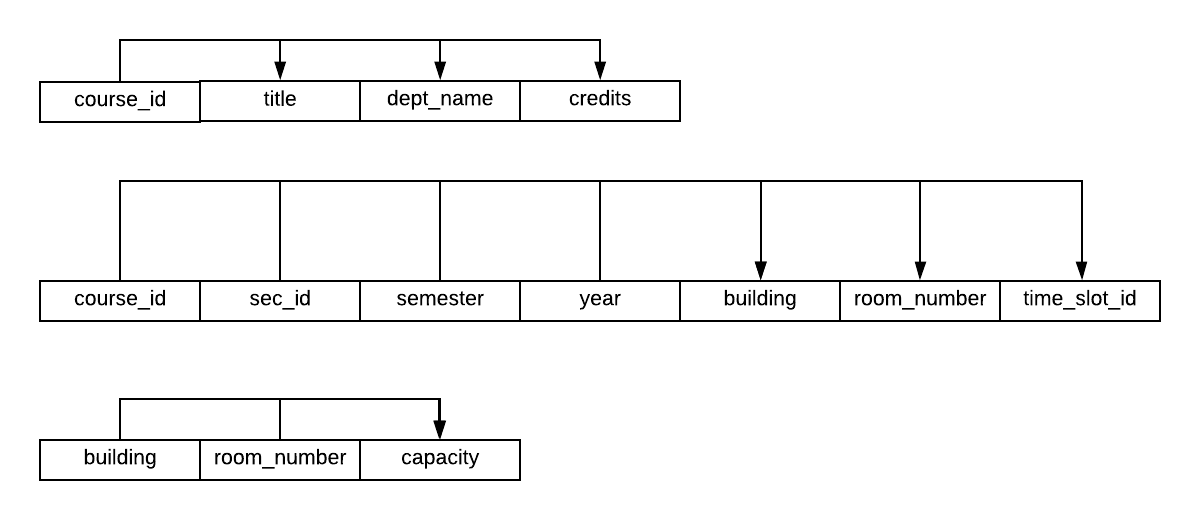
\includegraphics[width=1.0\textwidth, center]{images/3NF.png}

    
\end{enumerate}
\end{document}
